
\section{Tutorial project}
    The aim of the tutorial project is to provide an easy way to explore the IDE without reading long documents.
    The tutorial project can be opened from the [Main~Menu] -> [Help] -> [Tutorial~Project]. Demonstration project
    should introduce a new user into the basics of usage of this IDE, this generally covers the most common functions
    like assembling the code, running simulator, and so on.
    \begin{figure}[h]
        \centering{}
        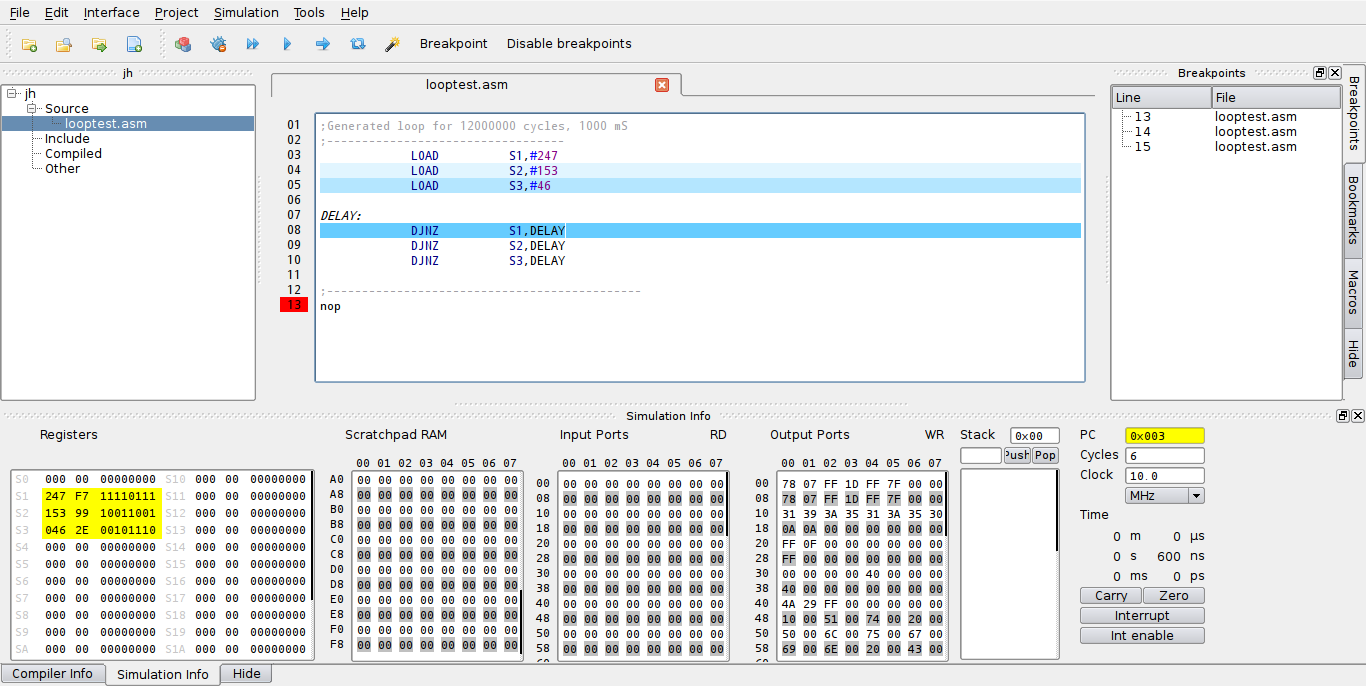
\includegraphics[width=\textwidth]{img/demonstration_1.png}
        \caption{Tutorial project}
    \end{figure}

\section{Your first project}
    There is not too much you have to do to start you first project in MDS, to keep things simple:
    \begin{itemize}
        \item Click on [Main~Menu] -> [Project] -> [New~Project].
        \item Choose a name for your project and directory in which you want to store files created in the IDE.
        \item On next tab you can adjust size of the scratch-pad and program memory, or change default interrupt vector.
        \item On Compiler tab you can choose files to generate by the assembler.
        \item Then click OK, and you have your project.
        \item Click on [Main~Menu] -> [File] -> [New~Project~File].
        \item Edit your file as you wish, and save it by clicking on [Main~Menu] -> [File] -> [Save~File].
    \end{itemize}

    \begin{table}[h!]
        \begin{tabular}{ccc}
            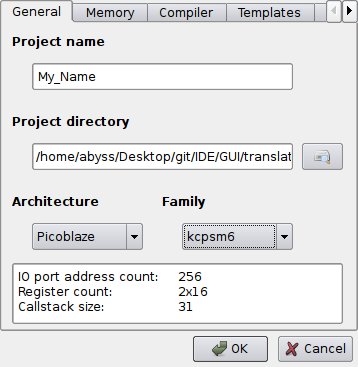
\includegraphics[width=.33\textwidth]{img/project_1.png}
                &
            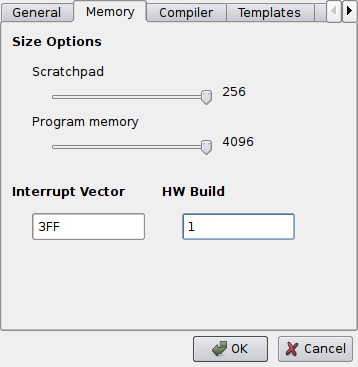
\includegraphics[width=.33\textwidth]{img/project_2.png}
                &
            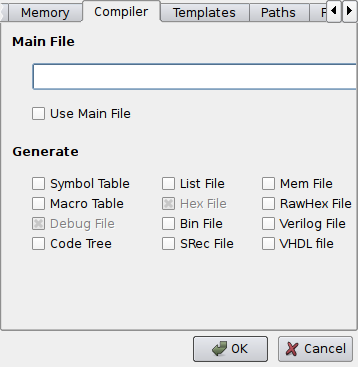
\includegraphics[width=.33\textwidth]{img/project_3.png}
                \\
            General & Memory & Compiler
        \end{tabular}
    \end{table}

    To use what you have just created:
    \begin{itemize}
        \item To assemble your file click on [Main~Menu] -> [Project] -> [Compile].
        \item To start simulation click on [Main~Menu] -> [Simulation] -> [Start~Simulation].
        \item Compiled files suitable for loading into FPGA can be found in the directory which you choose to be your
              project directory. Types of these files, and therefore their purpose, can be easily determined by their
              extensions\footnote{These file extensions are only recommended, the actual extensions can be set by user
              at any time.}:
            \begin{description}
                \item [.rawhex] is a raw hex file suitable for some JTAG loaders,
                \item [.mem] is a decimal representation of the machine code suitable for a number of various tools,
                \item [.ihex] is Intel 8 Hex,
                \item [.srec] is Motorola S-Record,
                \item [.bin] is plain binary file,
                \item [.lst] is code listing,
                \item [.stbl] is table of symbols,
                \item [.mtbl] is table of macros,
                \item [.dbg] is a file used the simulator for simulation, it has no other purpose,
                \item [.vhd] is VHDL code with your machine code (generated from template which can be chosen by user),
                \item [.v] is Verilog code with your machine code (generated from template which can be chosen by user),
                \item [.ctr] is so called code tree, this file has normally no application for regular users, it
                      contains textual representation of raw output from the syntax analyzer.
            \end{description}
    \end{itemize}
